%%This is a very basic article template.
%%There is just one section and two subsections.
\documentclass[12pt, twoside]{article}
\usepackage[francais]{babel}
\usepackage[T1]{fontenc}
\usepackage[latin1]{inputenc}
\usepackage[left=7mm, right=1cm, top=1cm, bottom=7mm]{geometry}
\usepackage{float}
\usepackage{graphicx}
\usepackage{array}
\usepackage{multirow}
\usepackage{amsmath,amssymb,mathrsfs}
\usepackage{soul}
\usepackage{textcomp}
\usepackage{eurosym}
 \usepackage{variations}
\usepackage{tabvar}
\pagestyle{empty}


\begin{document}


\ul{Conjecture} : Si un triangle est rectangle alors le centre du cercle circonscrit � ce triangle est le milieu de
l'hypot�nuse.


\bigskip

\begin{tabular}{cc}

\begin{minipage}{15cm}
\ul{D�monstration} : Tra�ons un triangle $GKH$ rectangle en $K$. Pla�ons $I$ le milieu de l'hypot�nuse $[GH]$.
Pla�ons le point $L$ sym�trique de $K$ par rapport � $I$.

\enskip

\fbox{
\begin{minipage}{12cm}
\ul{But} : On veut montrer que $I$ est bien le centre du cercle circonscrit au triangle $GKH$.
\end{minipage}
}

\end{minipage}
&
\begin{minipage}{3cm}
	\begin{center}
		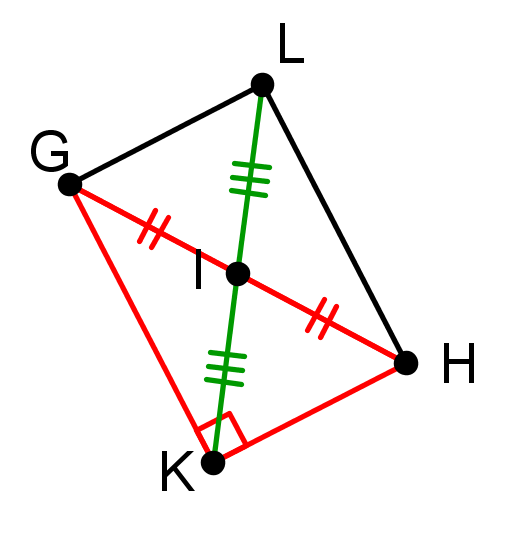
\includegraphics[width=3cm]{images/triangles-rectangles.png}
	\end{center}
\end{minipage}
\end{tabular}


\bigskip

\bigskip

\begin{itemize}
  \item[\ul{1� �tape}]\textit{: Montrons que $I$ est le milieu du segment $[KL]$}
  
  \enskip
  
  Donn�es : $L$ est le sym�trique de $K$ par rapport � $I$
  
  \enskip
  
  Propri�t� : Si $A'$ est le sym�trique du point $A$ par rapport au point $O$ alors $O$ est le milieu du segment
  $[AA']$.

  \enskip
  
  Conclusion : $I$ est le milieu du segment $[KL]$.
  
  
  \medskip
  
  \item[\ul{2� �tape}]\textit{: Montrons que $GKHL$ est un parall�logramme}
  
  \enskip
  
  Donn�es : \begin{itemize}
			  \item[$\bullet$] 
			  \item[$\bullet$] 
			\end{itemize}


  \enskip

  Propri�t� : Si un quadrilat�re a ses diagonales qui \ldots\ldots\ldots\ldots\ldots\ldots\ldots\ldots. \\ alors c'est
  un \ldots\ldots\ldots\ldots\ldots.
  
   \enskip
  
  Conclusion : 
  
  \medskip
  
  \item[\ul{3� �tape}]\textit{: Montrons que $GKHL$ est un rectangle}
  
  \enskip
  
  Donn�es : \begin{itemize}
			  \item[$\bullet$] 
			  \item[$\bullet$] 
            \end{itemize}
  
  \enskip
  
  Propri�t� : Si un parall�logramme poss�de un angle droit alors \ldots\ldots\ldots\ldots\ldots\ldots
  
  \enskip
  
  Conclusion : 
  
  
\medskip

  \item[\ul{4� �tape}]\textit{: Montrons que $IK=IG=IH$}
  
  \enskip

  Donn�es : \begin{itemize}
			  \item[$\bullet$] 
			  \item[$\bullet$] 
			\end{itemize}

  \enskip 

  Propri�t� : Si un quadrilat�re est un rectangle alors ses diagonales \ldots\ldots\ldots\ldots\ldots\ldots
  
  \enskip
  
  Conclusion : 
\end{itemize}

\end{document}
